\section{Divergence}

\subsection*{Overview}

A vector field has divergence when the vectors in that field point away from some point. Point-charges are a real-world example of this. We created a visualization of the electric field created by point charges to visually depict divergence. The field in the visualization has zero divergence everywhere except for where the point-charges lie. \cite{divergence1} \cite{divergence2}

\subsection*{Theoretical basis}

Given a vector field \(\vec E : \mathbb R^3 \to \mathbb R^3\), divergence \(\divf \vec E\) or \(\nabla \cdot \vec E\) is defined as \(\frac{\partial E_x}{\partial x} + \frac{\partial E_y}{\partial y} + \frac{\partial E_z}{\partial z}\). This describes whether the field \(E\) is a source or a sink.

Two point-charges attract by Coulomb's Law \(\vec F = \frac{1}{4 \pi \epsilon_0} \frac{q_1 q_2}{\|r\|^3} \;\vec r\). Let the first charge \(q_1\) be called the source and the second charge \(q_2\) the test-charge. Observe that \(\vec F = q_2 \vec E\), where \(E = \frac{1}{4 \pi \epsilon_0} \frac{q_1}{\|r\|^3} \;\vec r\). This field \(\vec E\) is useful because it abstracts out the test-charge. The field is only dependent on the source and the position.

When the source is centered around the origin, \(\vec E(x, y, z) = \frac{1}{4 \pi \epsilon_0 (x^2+y^2+z^2)^{3/2}} \; \langle x, y, z \rangle\). Since \(\frac{\partial E_x}{\partial x}\) is given by the quotient rule as \(\frac{-2x^2+y^2+z^2}{4 \pi \epsilon_0 (x^2+y^2+z^2)^{5/2}}\), \(\frac{\partial E_y}{\partial y}\) and \(\frac{\partial E_z}{\partial z}\) are similar, then the divergence at any point off of the origin is given by: \(\divf \vec E = \frac{1}{4 \pi \epsilon_0} \frac{(-2x^2 + y^2 + z^2) + (x^2 - 2y^2 + z^2) + (x^2 + y^2 - 2z^2)}{4 \pi \epsilon_0 (x^2 + y^2 + z^2)^{5/2}} = \vec 0\). For the origin, the divergence is undefined.

But it is given by Maxwell's equations that \(\iiint_S \divf \vec E \cdot \dif V = \frac{q}{\epsilon_0}\). Since \(\divf \vec E\) is zero everywhere except at the origin, and the integral is non-zero, the origin must be a Delta-Dirac function. A Delta-Dirac function \(\sigma (x)\) is defined such that \(\sigma (x) = 0\) everywhere except at \(x = 0\), when \(\sigma(x)\) is undefined, and \(\int_{-\infty}^\infty \sigma(x) \dif x = 1\).  Therefore \(\divf \vec E (0, 0, 0) = \frac{q}{\epsilon_0} \sigma(x)\sigma(y)\sigma(z)\), where \(\sigma(x)\) is the Delta-Dirac function.

Therefore electric fields have zero divergence except for at the point-charge which causes them. At that point, the divergence is infinite. The integral of the divergence of the electric field over a surface is just the number of charges contained in that surface.

\subsection*{Implementation details}

The electric fields are scaled by \(\frac{4 \pi \epsilon_0}{q}\), so that these constants do not appear in any part of the code.

The electric fields are generated from a curried function. A curried function is a function that returns another function. In this case, the \verb+field+ function inputs the location of a point-charge and outputs a function of \verb+x+, \verb+y+, and \verb+z+ which represents the vector field.

The actual vector arrows, if care is not taken, will be very large around the point-charge. This is because the point-charge creates a singularity where the magnitude of the electric field goes to infinity. To mitigate this, we ignore the vectors that are right near the point-charge and only plot the ones that are a certain distance away. This is done by the \verb+restrict+ function.

\subsection*{Usage notes}

This is intended to show students what divergence actually means. It doesn't just mean that the vector field is expanding, because in this vector field divergence is zero even though the arrows are going farther apart. The arrows are also getting smaller in length, which cancels out their expansion. The only divergence is caused by the point-charge itself, which has infinite divergence. This could be introduced at Lecture 34 Vector Fields and Curl after slide 7 which can give a more nuanced explanation to divergence.

It can also show Gauss' Law. Since \(\iiint_S \divf \vec E \dif \vec V\) is simply the number of point-charges, the left-hand side of Gauss' Law simplifies to the total charge \(q_T\) in \(q_T = \iint_{\partial S} \vec E \cdot \dif \vec S\). Instead of taking a volume-integral of divergence, you can literally count the number of point charges (count up for positive charges and down for negative ones). As such this animation could be revisited at Lecture 37 Gauss' Theorem as a motivating example before starting the presentation.

\begin{enumerate}
\item Set \verb+restriction[point_, radiusofrestriction_]+ to ignore the singularity.
\item Adjust \verb+opacity+ for viewing prefrences. It changes the transparency of the bounding sphere. 
\item Place point charges as a function of \verb+u+.
\item Set the bounds of \verb+u+ to be suitable to the function.
\end{enumerate}

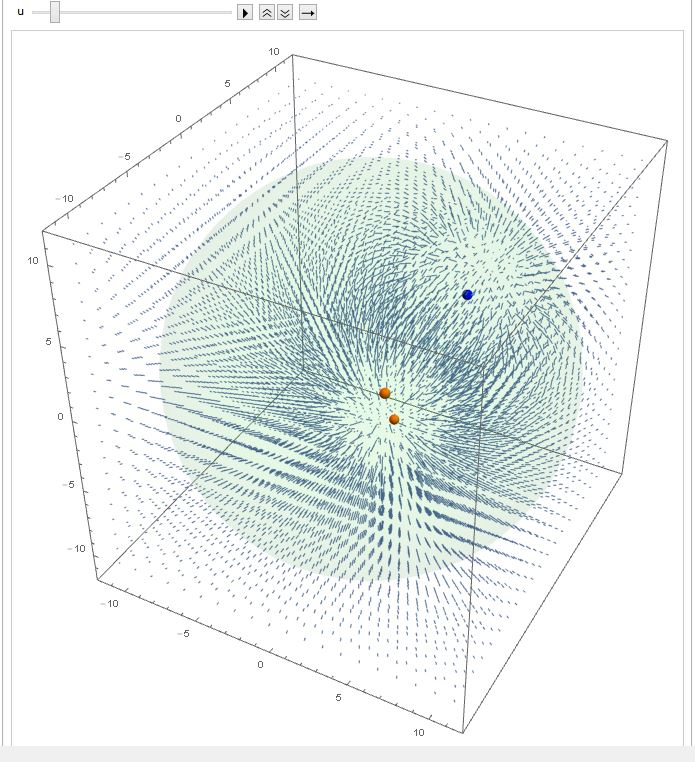
\includegraphics[height=16cm]{../exhibit/divergence.jpg}

%%% Local Variables:
%%% mode: latex
%%% TeX-master: "main"
%%% End:
